\documentclass[10pt]{article}
% \usepackage[UTF8]{ctex}

\usepackage[utf8]{inputenc} % allow utf-8 input
\usepackage{amsthm}
\usepackage{amsmath,amscd}
\usepackage{amssymb,array}
\usepackage{amsfonts,latexsym}
\usepackage{graphicx,subfig,wrapfig}
\usepackage{times}
\usepackage{psfrag,epsfig}
\usepackage{verbatim}
\usepackage{tabularx}
\usepackage[pagebackref=true,breaklinks=true,letterpaper=true,colorlinks,bookmarks=false]{hyperref}
\usepackage{cite}
\usepackage{algorithm}
\usepackage{multirow}
\usepackage{caption}
\usepackage{algorithmic}
%\usepackage[amsmath,thmmarks]{ntheorem}
\usepackage{color}
\usepackage{bm}

% -------------------------------------------------------------------------------------
% \usepackage[UTF8]{ctex} % 显示中文
\usepackage{CJK}
\usepackage{xcolor} 
\usepackage{listings}
\lstset{%
	alsolanguage=Java,
	%alsolanguage=[ANSI]C,      %可以添加很多个alsolanguage,如alsolanguage=matlab,alsolanguage=VHDL等
	alsolanguage= matlab,
	alsolanguage= XML,
	tabsize=4, %
	frame=shadowbox, %把代码用带有阴影的框圈起来
	commentstyle=\color{red!50!green!50!blue!50},%浅灰色的注释
	rulesepcolor=\color{red!20!green!20!blue!20},%代码块边框为淡青色
	keywordstyle=\color{blue!90}\bfseries, %代码关键字的颜色为蓝色,粗体
	showstringspaces=false,%不显示代码字符串中间的空格标记
	stringstyle=\ttfamily, % 代码字符串的特殊格式
	keepspaces=true, %
	breakindent=22pt, %
	numbers=left,%左侧显示行号 往左靠,还可以为right,或none,即不加行号
	stepnumber=1,%若设置为2,则显示行号为1,3,5,即stepnumber为公差,默认stepnumber=1
	%numberstyle=\tiny, %行号字体用小号
	numberstyle={\color[RGB]{0,192,192}\tiny} ,%设置行号的大小,大小有tiny,scriptsize,footnotesize,small,normalsize,large等
	numbersep=8pt,  %设置行号与代码的距离,默认是5pt
	basicstyle=\footnotesize, % 这句设置代码的大小
	showspaces=false, %
	flexiblecolumns=true, %
	breaklines=true, %对过长的代码自动换行
	breakautoindent=true,%
	breakindent=4em, %
	escapebegin=\begin{CJK*}{GBK}{hei},escapeend=\end{CJK*},
	aboveskip=1em, %代码块边框
	tabsize=2,
	showstringspaces=false, %不显示字符串中的空格
	backgroundcolor=\color[RGB]{245,245,244},   %代码背景色
	%backgroundcolor=\color[rgb]{0.91,0.91,0.91}    %添加背景色
	escapeinside=``,  %在``里显示中文
	%% added by http://bbs.ctex.org/viewthread.php?tid=53451
	fontadjust,
	captionpos=t,
	framextopmargin=2pt,framexbottommargin=2pt,abovecaptionskip=-3pt,belowcaptionskip=3pt,
	xleftmargin=4em,xrightmargin=4em, % 设定listing左右的空白
	% 设定中文冲突,断行,列模式,数学环境输入,listing数字的样式
	extendedchars=false,columns=flexible,mathescape=true
	% numbersep=-1em
}

% -------------------------------------------------------------------------------------



\newtheorem{thm}{Theorem}
\newtheorem{mydef}{Definition}

\DeclareMathOperator*{\rank}{rank}
\DeclareMathOperator*{\trace}{trace}
\DeclareMathOperator*{\acos}{acos}
\DeclareMathOperator*{\argmax}{argmax}


\renewcommand{\algorithmicrequire}{ \textbf{Input:}}
\renewcommand{\algorithmicensure}{ \textbf{Output:}}
\renewcommand{\mathbf}{\boldsymbol}
\newcommand{\mb}{\mathbf}
\newcommand{\matlab}[1]{\texttt{#1}}
\newcommand{\setname}[1]{\textsl{#1}}  
\newcommand{\Ce}{\mathbb{C}}
\newcommand{\Ee}{\mathbb{E}}
\newcommand{\Ne}{\mathbb{N}}
\newcommand{\Se}{\mathbb{S}}
\newcommand{\norm}[2]{\left\| #1 \right\|_{#2}}

\newenvironment{mfunction}[1]{
	\noindent
	\tabularx{\linewidth}{>{\ttfamily}rX}
	\hline
	\multicolumn{2}{l}{\textbf{Function \matlab{#1}}}\\
	\hline
}{\\\endtabularx}

\newcommand{\parameters}{\multicolumn{2}{l}{\textbf{Parameters}}\\}

\newcommand{\fdescription}[1]{\multicolumn{2}{p{0.96\linewidth}}{

		\textbf{Description}

		#1}\\\hline}

\newcommand{\retvalues}{\multicolumn{2}{l}{\textbf{Returned values}}\\}
\def\0{\boldsymbol{0}}
\def\b{\boldsymbol{b}}
\def\bmu{\boldsymbol{\mu}}
\def\e{\boldsymbol{e}}
\def\u{\boldsymbol{u}}
\def\x{\boldsymbol{x}}
\def\v{\boldsymbol{v}}
\def\w{\boldsymbol{w}}
\def\N{\boldsymbol{N}}
\def\X{\boldsymbol{X}}
\def\Y{\boldsymbol{Y}}
\def\A{\boldsymbol{A}}
\def\B{\boldsymbol{B}}
\def\y{\boldsymbol{y}}
\def\cX{\mathcal{X}}
\def\transpose{\top} % Vector and Matrix Transpose

%\long\def\answer#1{{\bf ANSWER:} #1}
\long\def\answer#1{}
\newcommand{\myhat}{\widehat}
\long\def\comment#1{}
\newcommand{\eg}{{e.g.,~}}
\newcommand{\ea}{{et al.~}}
\newcommand{\ie}{{i.e.,~}}

\newcommand{\db}{{\boldsymbol{d}}}
\renewcommand{\Re}{{\mathbb{R}}}
\newcommand{\Pe}{{\mathbb{P}}}
\newenvironment{problem}[2][Problem]{\begin{trivlist}
\item[\hskip \labelsep {\bfseries #1}\hskip \labelsep {\bfseries #2.}]}{\end{trivlist}}

\hyphenation{MATLAB}

\usepackage[margin=1in]{geometry}

\begin{document}

\title{	Numerical Optimization, 2023 Fall\\Homework 4}
\date{Due 23:59 (CST), Jan. 4, 2024 }

\author{
    Name: \textbf{Zhou Shouchen} \\
	Student ID: 2021533042
}

\maketitle
\newpage

% %===============================

\begin{problem}{1}
    $f$ is a positive definite quadratic function $$f(\pmb x) = \frac{1}{2}\pmb x^T\pmb A\pmb x + \pmb b^T\pmb x,  \quad \pmb A \in \mathbb{S}_{++}^n, \pmb b \in \mathbb{R}^n,$$ $\pmb x^k$ is the current iteration point, $\pmb d^k$ is the descent direction. Derive the step size of exact linear search \textcolor{red}{[20pts]} $$\alpha^k = \arg\min_{\alpha > 0}f(\pmb x^k + \alpha \pmb d^k).$$
\end{problem}

Let $g(\alpha)=f(\pmb x^k+\alpha\pmb d^k)=\dfrac{1}{2}(\pmb x^k+\alpha\pmb d^k)^T\pmb A(\pmb x^k+\alpha\pmb d^k)+\pmb b^T(\pmb x^k+\alpha\pmb d^k)$.\\
So $$\dfrac{\partial g}{\partial \alpha}=\alpha(\pmb d^k)^T\pmb A\pmb d^k+\dfrac{1}{2}(\pmb d^k)^T\pmb A\pmb x^k+\dfrac{1}{2}(\pmb x^k)^T\pmb A\pmb d^k+\pmb b^T\pmb d^k$$
Since $\pmb A\in \mathbb{S}_{++}^n$, i.e. $\pmb A$ is symmetric, so $$(\pmb d^k)^T\pmb A\pmb x^k=(\pmb x^k)^T\pmb A\pmb d^k$$
So $$\dfrac{\partial g}{\partial\alpha}=\alpha(\pmb d^k)^T\pmb A\pmb d^k+(\pmb d^k)^T\pmb A\pmb x^k+\pmb b^T\pmb d^k$$
And $$\dfrac{\partial^2 g}{\partial\alpha^2}=(\pmb d^k)^T\pmb A\pmb d^k$$
Since $\pmb A\in \mathbb{S}_{++}^n$, which means that $\pmb A$ is a positive defined matrix, i.e. 
$$\forall \pmb x\in \mathbb{R}^n, \pmb x^T\pmb A\pmb x>0$$
So $$\forall\pmb d^k, \dfrac{\partial^2 g}{\partial\alpha^2}=(\pmb d^k)^T\pmb A\pmb d^k>0$$
So $g(\alpha)$ is a convex function. In order to find the minimum point $\alpha^k = \arg\min\limits_{\alpha > 0}g(\alpha)$, we just need to let the gradient to be $0$.
i.e. $$\dfrac{\partial g}{\partial\alpha}(\alpha^k)=0$$
So $$\alpha^k(\pmb d^k)^T\pmb A\pmb d^k+(\pmb d^k)^T\pmb A\pmb x^k+\pmb b^T\pmb d^k=0$$
So $$\alpha^k = -\dfrac{((\pmb d^k)^T\pmb A\pmb x^k+\pmb b^T\pmb d^k)}{(\pmb d^k)^T\pmb A\pmb d^k}$$
Since we have known that $(\pmb d^k)^T\pmb A\pmb d^k>0$, so the $\alpha^k$ is a legal solution.\\
So abovel all, the step size of exact linear search is
$$\alpha^k = -\dfrac{((\pmb d^k)^T\pmb A\pmb x^k+\pmb b^T\pmb d^k)}{(\pmb d^k)^T\pmb A\pmb d^k}$$

\newpage
% %===============================

\begin{problem}{2}
    Prove that $f: \mathbb{R}^n \rightarrow \mathbb{R}$ is affine if and only if $f$ is both convex and concave. \textcolor{red}{[20pts]} 
\end{problem}

1. sufficiency:\\
If $f$ is affine, then we can write $f$ as $f(\pmb x)=\pmb w^{\top}\pmb x+b$, where $\pmb w\in \mathbb{R}^n, b\in \mathbb{R}$.\\
Then we have $$\nabla f(\pmb x)=\pmb w$$
and $$\nabla^2 f(\pmb x)=\pmb 0$$
So
$$\nabla^2 f(\pmb x) \succeq \pmb 0, \nabla^2 f(\pmb x) \preceq \pmb 0$$
So $f$ is both convex and concave.\\

2. necessity:\\
If $f$ is convex and concave, then we have:\\
since $f$ is concave, so $$\forall \pmb x_1,\pmb x_2, \theta\in [0,1], f(\theta\pmb x_1+(1-\theta)\pmb x_2)\geq \theta f(\pmb x_1)+(1-\theta)f(\pmb x_2)$$
since $f$ is convex, so $$\forall \pmb x_1,\pmb x_2, \theta\in [0,1], f(\theta\pmb x_1+(1-\theta)\pmb x_2)\leq \theta f(\pmb x_1)+(1-\theta)f(\pmb x_2)$$
So we have $$\forall \pmb x_1,\pmb x_2, \theta\in [0,1], f(\theta\pmb x_1+(1-\theta)\pmb x_2)= \theta f(\pmb x_1)+(1-\theta)f(\pmb x_2)$$
Which is exactly the definition of affine function.\\
So $f$ is affine.\\
 
So above all, we have proved that $f:\mathbb{R}^n\rightarrow \mathbb{R}$ is affine if and only if $f$ is both convex and concave.

\newpage
%===============================

\begin{problem}{3}
    Solve the optimal solution of the Rosenbrock function $$f(x, y) = (1 - x)^2 + 100(y - x^2)^2, $$ using MATLAB programming to implement three algorithms (each 20pts): gradient descent (GD) method, Newton method, and Quasi-Newton methods (either rank-1, DFP or BFGS). You are required to print iteration information of last 10 steps: including objective, step size, residual of gradient. Technical implementation: explain how to choose the step size, how to set the termination criteria, how to choose the initial point, the value of the required parameters, converge or not and convergence rate. (paste the code in the pdf to submit it, no need to submit the source code) \textcolor{red}{[60pts]}
\end{problem}

1. Gradient descent method:\\
set step size to be constant: $\alpha^k=0.002$.\\
direction: $\pmb d^k=-\nabla f(\pmb x^k)$.\\
The update policy: following the direction of the negative gradient, i.e.
$$\pmb x^{k+1}=\pmb x^k-\alpha^k\nabla f(\pmb x^k)$$
termination criteria: if the current point's gradiant's norm $\norm{\nabla f(\pmb x^k)}{2}<10^{-4}$, then we regard it converges.
initial point: $\pmb x^0=(x,y)$, where $x$ and $y$ are randomly uniformed generated in the range $[-1,1]$.\\
There is no additional parameters.\\
The method converged, and from the variation of output, we can see that the convergence rate is linear convergence.\\

2. Newton method:\\
step size: $\alpha^k=1$.\\
direction: $\pmb d^k = -\nabla^2 f(\pmb x^k)^{-1}\nabla f(\pmb x^k)$.\\
The update policy: find the zero point of the first order derivative, and then update the current point to the interaction point of the current point's tangent line and the axis, i.e.
$$\pmb x^{k+1}=\pmb x^k-\nabla^2 f(\pmb x^k)^{-1}\nabla f(\pmb x^k)$$
termination criteria: if the current point's gradiant's norm $\norm{\nabla f(\pmb x^k)}{2}<10^{-4}$, then we regard it converges.
initial point: $\pmb x^0=(x,y)$, where $x$ and $y$ are randomly uniformed generated in the range $[-1,1]$.\\
There is no additional parameters.\\
The method converged, and from the variation of output, we can see that the convergence rate is quadratic convergence.\\

3. Quasi-Newton method:\\
step size: we can use Armijo linear seach to find a suitable $\alpha^k$: setting $\alpha^k=1$, and $\gamma=0.5$, and let $\alpha^k$ constantly times $\gamma$ until the Armijo condition: $f(\pmb x^k+\alpha^k\pmb d^k)\leq f(\pmb x^k)+\alpha^k\gamma\nabla f(\pmb x^k)^T\pmb d^k$ is satisfied.\\
direction: $\pmb d^k = -H_k^{-1}\nabla f(\pmb x^k)$, where $H_k$ is generated by BFGS method.\\
The update policy: similarly to Newton-method, but do not directly get the Hessian matrix but construct a similar $H_k$, and then update the current point to the interaction point of the current point and last point's secant line and the axis, i.e.
$$\pmb x^{k+1}=\pmb x^k-\alpha^kH_k^{-1}\nabla f(\pmb x^k)$$
termination criteria: if the current point's gradiant's norm $\norm{\nabla f(\pmb x^k)}{2}<10^{-4}$, then we regard it converges.
initial point: $\pmb x^0=(x,y)$, where $x$ and $y$ are randomly uniformed generated in the range $[-1,1]$.\\
The original $H_0^{-1}$ is set to be $I_2$.\\
As for the update of $H_k^{-1}$, we set $\pmb s_k=\pmb x^{k+1}-\pmb x^k$ and $\pmb y^k=\nabla f(\pmb x^{k+1})-\nabla f(\pmb x^k)$, and we use the BFGS method to update $H_k^{-1}$.\\
i.e. if ${\pmb s_k}^{\top}{\pmb y_k}>0$, then we update $H_{k+1}^{-1}=(I_2-\dfrac{{\pmb s_k}{\pmb y_k}^{\top}}{{\pmb y_k}^{\top}{\pmb s_k}})H_k^{-1}(I_2-\dfrac{{\pmb y_k}{\pmb s_k}^{\top}}{{\pmb y_k}^{\top}{\pmb s_k}})+\dfrac{{\pmb s_k}{\pmb s_k}^{\top}}{{\pmb y_k}^{\top}{\pmb s_k}}$.\\
Ohterwise it remains: $H_{k+1}^{-1}=H_k^{-1}$.\\
The method converged, and from the variation of output, we can see that the convergence rate is superlinear convergence.\\

The output information and the trace of the three methods are as follows(it seems that the format of output is not aligned in latex, but it worked well in matlab file...):

\begin{figure}[htbp]
	\centering
	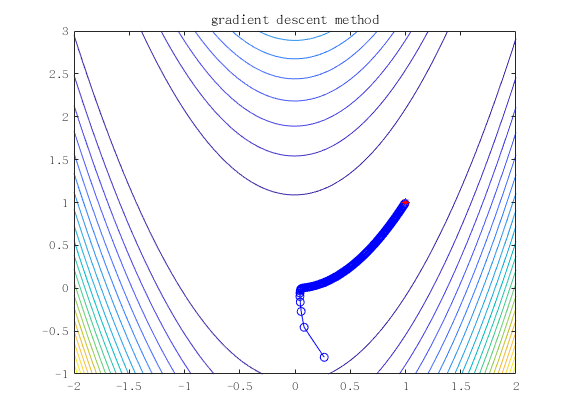
\includegraphics[width=0.32\textwidth]{../code/result/gradient_descent.png}
	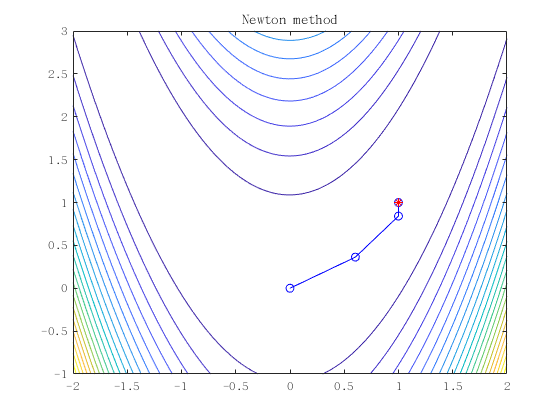
\includegraphics[width=0.32\textwidth]{../code/result/Newton_method.png}
	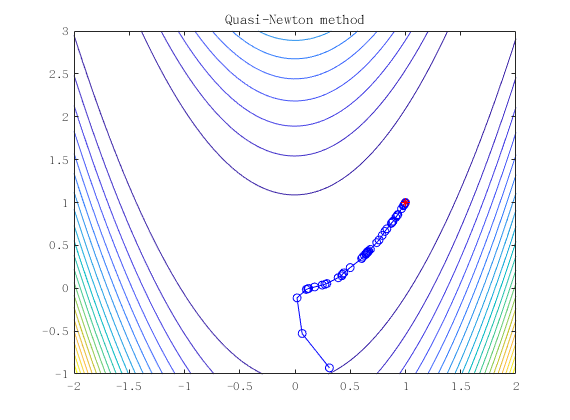
\includegraphics[width=0.32\textwidth]{../code/result/Quasi_Newton_method.png}
\end{figure}

\lstinputlisting[title=output]{../code/output.txt}

And the codes are as follows:\\

\lstinputlisting[title=Rosenbrock.m, language=matlab]{../code/Rosenbrock.m}
	
\lstinputlisting[title=print\_info.m, language=matlab]{../code/print_info.m}

\lstinputlisting[title=plot\_trace.m, language=matlab]{../code/plot_trace.m}

\lstinputlisting[title=gradient\_descent.m, language=matlab]{../code/gradient_descent.m}

\lstinputlisting[title=Newton\_method.m, language=matlab]{../code/Newton_method.m}

\lstinputlisting[title=Quasi\_Newton\_method.m, language=matlab]{../code/Quasi_Newton_method.m}

\lstinputlisting[title=implement.m, language=matlab]{../code/implement.m}

\end{document}
